% Fig. 3.16 -- 迴歸函數 E(X|Y=y) 在曲面上的位置。
% 書稿來源: mathstatch3.tex 第 2297 至 2348 行的 tikzpicture (單面板)。
%
% 幾何一律照書稿: view={50}{45}、width=11cm、domain 0:4、y domain 0:4、
% 座標軸線不畫、x 軸與鉛直軸都不標刻度; y 軸三個刻度在 0.7、1.5 與 3，
% 依序標 y_1、y_2 與 y_n。三片切面即在這三個 y 上沿 x 方向的截面。
% 曲面照書稿自定的 bivar 函數，取 mu1=mu2=2、sigma1=sigma2=1; 指數部分沒有
% 慣見的 1/2，整體另外再除以 2，與 Fig. 3.2、Fig. 3.11 是同一條式子。
%
% 對書稿的四處調整:
%   1. colormap 由 whitegray 改為同色相的墨色濃淡 journalgray (CH3 規格 3.2)。
%   2. samples 由 50 改為 40 (CH3 規格 3.2 所定的產製規格)。
%   3. 三片切面的填色由 fill=gray、opacity=0.4 改為 journalaccent、
%      fill opacity=0.15 (CH3 規格第一節)，切面曲線 journalink 0.8pt，
%      填色區的外框走 journalmuted 0.5pt。
%   4. 字級: 書稿的 $f_{\sssig XY}$ 走 scriptscriptstyle，350px 顯示寬之下
%      下標不足 11px 門檻。此處改為一般下標，字級一律 \large，並以
%      \DeclareMathSizes 把 12pt 之下的 script 級撐到 10pt。
%
% 另有一處書稿沒有處理的瑕疵: 座標軸線設為不畫之後，pgfplots 預設的框線刻度
% 仍會在遠端浮出三個孤立的短記號 (書稿原圖左上角即可見)，此處以
% tick style={draw=none} 一併關掉，刻度標示不受影響。
%
% 量測: viewBox 寬 266.97，350px 之下放大 1.311 倍;
% 最小可見字為 10pt 的下標 (9.96 SVG 單位)，合 13.1px，在 11px 門檻之上。
%
% 產製 (CH3 規格 3.2 的三維曲面路徑，-O 不可省):
%   latex -interaction=nonstopmode '\def\pgfsysdriver{pgfsys-dvisvgm.def}% Fig. 3.16 -- 迴歸函數 E(X|Y=y) 在曲面上的位置。
% 書稿來源: mathstatch3.tex 第 2297 至 2348 行的 tikzpicture (單面板)。
%
% 幾何一律照書稿: view={50}{45}、width=11cm、domain 0:4、y domain 0:4、
% 座標軸線不畫、x 軸與鉛直軸都不標刻度; y 軸三個刻度在 0.7、1.5 與 3，
% 依序標 y_1、y_2 與 y_n。三片切面即在這三個 y 上沿 x 方向的截面。
% 曲面照書稿自定的 bivar 函數，取 mu1=mu2=2、sigma1=sigma2=1; 指數部分沒有
% 慣見的 1/2，整體另外再除以 2，與 Fig. 3.2、Fig. 3.11 是同一條式子。
%
% 對書稿的四處調整:
%   1. colormap 由 whitegray 改為同色相的墨色濃淡 journalgray (CH3 規格 3.2)。
%   2. samples 由 50 改為 40 (CH3 規格 3.2 所定的產製規格)。
%   3. 三片切面的填色由 fill=gray、opacity=0.4 改為 journalaccent、
%      fill opacity=0.15 (CH3 規格第一節)，切面曲線 journalink 0.8pt，
%      填色區的外框走 journalmuted 0.5pt。
%   4. 字級: 書稿的 $f_{\sssig XY}$ 走 scriptscriptstyle，350px 顯示寬之下
%      下標不足 11px 門檻。此處改為一般下標，字級一律 \large，並以
%      \DeclareMathSizes 把 12pt 之下的 script 級撐到 10pt。
%
% 另有一處書稿沒有處理的瑕疵: 座標軸線設為不畫之後，pgfplots 預設的框線刻度
% 仍會在遠端浮出三個孤立的短記號 (書稿原圖左上角即可見)，此處以
% tick style={draw=none} 一併關掉，刻度標示不受影響。
%
% 量測: viewBox 寬 266.97，350px 之下放大 1.311 倍;
% 最小可見字為 10pt 的下標 (9.96 SVG 單位)，合 13.1px，在 11px 門檻之上。
%
% 產製 (CH3 規格 3.2 的三維曲面路徑，-O 不可省):
%   latex -interaction=nonstopmode '\def\pgfsysdriver{pgfsys-dvisvgm.def}% Fig. 3.16 -- 迴歸函數 E(X|Y=y) 在曲面上的位置。
% 書稿來源: mathstatch3.tex 第 2297 至 2348 行的 tikzpicture (單面板)。
%
% 幾何一律照書稿: view={50}{45}、width=11cm、domain 0:4、y domain 0:4、
% 座標軸線不畫、x 軸與鉛直軸都不標刻度; y 軸三個刻度在 0.7、1.5 與 3，
% 依序標 y_1、y_2 與 y_n。三片切面即在這三個 y 上沿 x 方向的截面。
% 曲面照書稿自定的 bivar 函數，取 mu1=mu2=2、sigma1=sigma2=1; 指數部分沒有
% 慣見的 1/2，整體另外再除以 2，與 Fig. 3.2、Fig. 3.11 是同一條式子。
%
% 對書稿的四處調整:
%   1. colormap 由 whitegray 改為同色相的墨色濃淡 journalgray (CH3 規格 3.2)。
%   2. samples 由 50 改為 40 (CH3 規格 3.2 所定的產製規格)。
%   3. 三片切面的填色由 fill=gray、opacity=0.4 改為 journalaccent、
%      fill opacity=0.15 (CH3 規格第一節)，切面曲線 journalink 0.8pt，
%      填色區的外框走 journalmuted 0.5pt。
%   4. 字級: 書稿的 $f_{\sssig XY}$ 走 scriptscriptstyle，350px 顯示寬之下
%      下標不足 11px 門檻。此處改為一般下標，字級一律 \large，並以
%      \DeclareMathSizes 把 12pt 之下的 script 級撐到 10pt。
%
% 另有一處書稿沒有處理的瑕疵: 座標軸線設為不畫之後，pgfplots 預設的框線刻度
% 仍會在遠端浮出三個孤立的短記號 (書稿原圖左上角即可見)，此處以
% tick style={draw=none} 一併關掉，刻度標示不受影響。
%
% 量測: viewBox 寬 266.97，350px 之下放大 1.311 倍;
% 最小可見字為 10pt 的下標 (9.96 SVG 單位)，合 13.1px，在 11px 門檻之上。
%
% 產製 (CH3 規格 3.2 的三維曲面路徑，-O 不可省):
%   latex -interaction=nonstopmode '\def\pgfsysdriver{pgfsys-dvisvgm.def}% Fig. 3.16 -- 迴歸函數 E(X|Y=y) 在曲面上的位置。
% 書稿來源: mathstatch3.tex 第 2297 至 2348 行的 tikzpicture (單面板)。
%
% 幾何一律照書稿: view={50}{45}、width=11cm、domain 0:4、y domain 0:4、
% 座標軸線不畫、x 軸與鉛直軸都不標刻度; y 軸三個刻度在 0.7、1.5 與 3，
% 依序標 y_1、y_2 與 y_n。三片切面即在這三個 y 上沿 x 方向的截面。
% 曲面照書稿自定的 bivar 函數，取 mu1=mu2=2、sigma1=sigma2=1; 指數部分沒有
% 慣見的 1/2，整體另外再除以 2，與 Fig. 3.2、Fig. 3.11 是同一條式子。
%
% 對書稿的四處調整:
%   1. colormap 由 whitegray 改為同色相的墨色濃淡 journalgray (CH3 規格 3.2)。
%   2. samples 由 50 改為 40 (CH3 規格 3.2 所定的產製規格)。
%   3. 三片切面的填色由 fill=gray、opacity=0.4 改為 journalaccent、
%      fill opacity=0.15 (CH3 規格第一節)，切面曲線 journalink 0.8pt，
%      填色區的外框走 journalmuted 0.5pt。
%   4. 字級: 書稿的 $f_{\sssig XY}$ 走 scriptscriptstyle，350px 顯示寬之下
%      下標不足 11px 門檻。此處改為一般下標，字級一律 \large，並以
%      \DeclareMathSizes 把 12pt 之下的 script 級撐到 10pt。
%
% 另有一處書稿沒有處理的瑕疵: 座標軸線設為不畫之後，pgfplots 預設的框線刻度
% 仍會在遠端浮出三個孤立的短記號 (書稿原圖左上角即可見)，此處以
% tick style={draw=none} 一併關掉，刻度標示不受影響。
%
% 量測: viewBox 寬 266.97，350px 之下放大 1.311 倍;
% 最小可見字為 10pt 的下標 (9.96 SVG 單位)，合 13.1px，在 11px 門檻之上。
%
% 產製 (CH3 規格 3.2 的三維曲面路徑，-O 不可省):
%   latex -interaction=nonstopmode '\def\pgfsysdriver{pgfsys-dvisvgm.def}\input{regression-function-surface.tex}'
%   dvisvgm -O -d2 -n -o ../../images/teaching-topics/regression-function-surface.svg regression-function-surface.dvi

\documentclass[tikz,border=2pt]{standalone}
\usepackage{amsmath}
\usepackage{amssymb}
\usepackage{xcolor}
\usepackage{pgfplots}
\pgfplotsset{compat=1.18}

\definecolor{journalink}{HTML}{1F1C18}
\definecolor{journalmuted}{HTML}{8A7F72}
\definecolor{journalaccent}{HTML}{9C2D2D}

%% 12pt (即 \large) 之下的 script 級撐到 10pt，
%% 使 f 的下標與 y 的下標在 350px 顯示寬之下仍在 11px 之上。
\DeclareMathSizes{12}{12}{10}{8}

%% 書稿用 whitegray 灰階曲面; 本站改用同一色相的墨色濃淡，
%% 與其他圖的主線色 journalink 相稱。
\pgfplotsset{
  colormap={journalgray}{color(0cm)=(white); color(1cm)=(journalink)}
}

\begin{document}
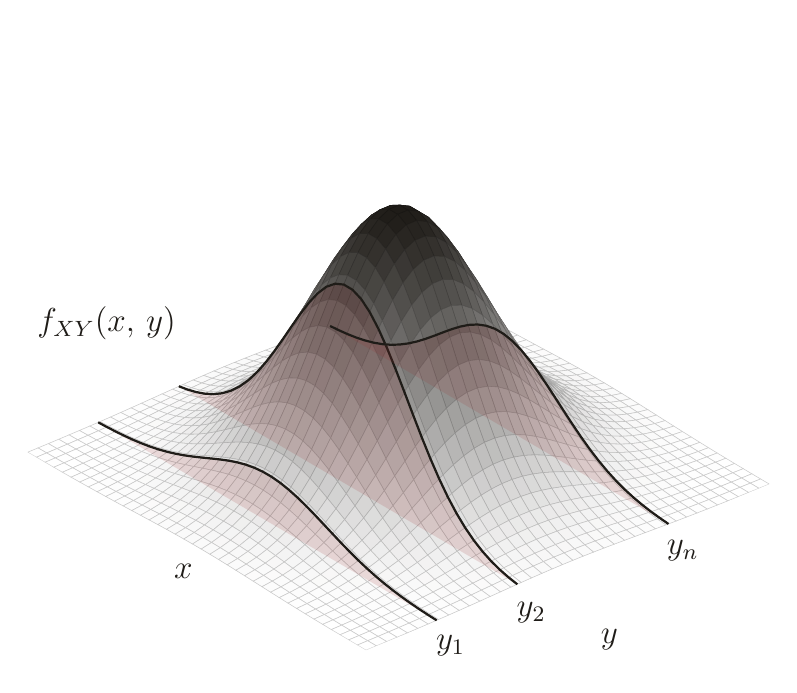
\begin{tikzpicture}[
    declare function={mu1=2;},
    declare function={mu2=2;},
    declare function={sigma1=1;},
    declare function={sigma2=1;},
    declare function={bivar(\ma,\sa,\mb,\sb)=
        1/(2*pi*\sa*\sb) * exp(-((x-\ma)^2/\sa^2 + (y-\mb)^2/\sb^2))/2;},
    declare function={slice(\yy)=
        1/(2*pi) * exp(-((x-2)^2 + (\yy-2)^2))/2;}]
\begin{axis}[
    axis line style={draw=none},
    colormap name=journalgray,
    width=11cm,
    view={50}{45},
    enlargelimits=false,
    domain=0:4,
    y domain=0:4,
    samples=40,
    xlabel=$x$,
    ylabel=$y$,
    zlabel={$f_{XY}(x,\,y)$},
    label style={journalink, font=\large},
    tick label style={journalink, font=\large},
    %% 座標軸線不畫，預設的框線刻度會在遠端浮成三個孤立的短記號，故一併關掉
    tick style={draw=none},
    xtick=\empty,
    ytick={0.7, 1.5, 3},
    yticklabels={$y_1$, $y_2$, $y_n$},
    ztick=\empty,
    zlabel style={rotate=-90, anchor=west},
]
\addplot3[surf, draw=journalink, line width=0.2pt] {bivar(mu1,sigma1,mu2,sigma2)};

%% 三片薄片: 每一片是聯合 pdf 在該 y 上沿 x 方向的截面，
%% 即 X 給定 Y=y 的條件分配 (尚未除以邊際密度)。
\addplot3[domain=0:4, samples y=0, samples=40, draw=journalmuted,
          line width=0.5pt, fill=journalaccent, fill opacity=0.15]
         (x, 0.7, {slice(0.7)});
\addplot3[domain=0:4, samples y=0, samples=40, journalink, line width=0.8pt]
         (x, 0.7, {slice(0.7)});

\addplot3[domain=0:4, samples y=0, samples=40, draw=journalmuted,
          line width=0.5pt, fill=journalaccent, fill opacity=0.15]
         (x, 1.5, {slice(1.5)});
\addplot3[domain=0:4, samples y=0, samples=40, journalink, line width=0.8pt]
         (x, 1.5, {slice(1.5)});

\addplot3[domain=0:4, samples y=0, samples=40, draw=journalmuted,
          line width=0.5pt, fill=journalaccent, fill opacity=0.15]
         (x, 3, {slice(3)});
\addplot3[domain=0:4, samples y=0, samples=40, journalink, line width=0.8pt]
         (x, 3, {slice(3)});
\end{axis}
\end{tikzpicture}
\end{document}
'
%   dvisvgm -O -d2 -n -o ../../images/teaching-topics/regression-function-surface.svg regression-function-surface.dvi

\documentclass[tikz,border=2pt]{standalone}
\usepackage{amsmath}
\usepackage{amssymb}
\usepackage{xcolor}
\usepackage{pgfplots}
\pgfplotsset{compat=1.18}

\definecolor{journalink}{HTML}{1F1C18}
\definecolor{journalmuted}{HTML}{8A7F72}
\definecolor{journalaccent}{HTML}{9C2D2D}

%% 12pt (即 \large) 之下的 script 級撐到 10pt，
%% 使 f 的下標與 y 的下標在 350px 顯示寬之下仍在 11px 之上。
\DeclareMathSizes{12}{12}{10}{8}

%% 書稿用 whitegray 灰階曲面; 本站改用同一色相的墨色濃淡，
%% 與其他圖的主線色 journalink 相稱。
\pgfplotsset{
  colormap={journalgray}{color(0cm)=(white); color(1cm)=(journalink)}
}

\begin{document}
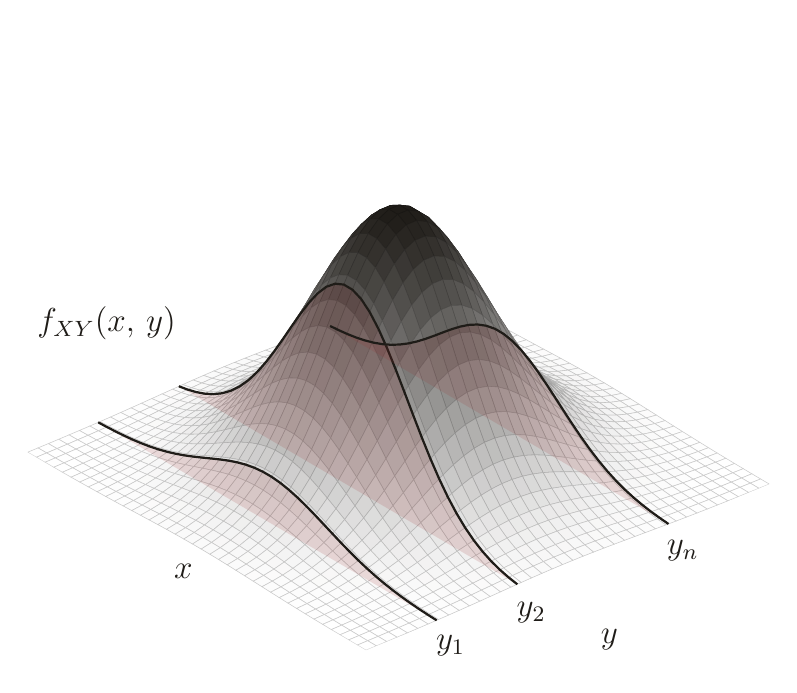
\begin{tikzpicture}[
    declare function={mu1=2;},
    declare function={mu2=2;},
    declare function={sigma1=1;},
    declare function={sigma2=1;},
    declare function={bivar(\ma,\sa,\mb,\sb)=
        1/(2*pi*\sa*\sb) * exp(-((x-\ma)^2/\sa^2 + (y-\mb)^2/\sb^2))/2;},
    declare function={slice(\yy)=
        1/(2*pi) * exp(-((x-2)^2 + (\yy-2)^2))/2;}]
\begin{axis}[
    axis line style={draw=none},
    colormap name=journalgray,
    width=11cm,
    view={50}{45},
    enlargelimits=false,
    domain=0:4,
    y domain=0:4,
    samples=40,
    xlabel=$x$,
    ylabel=$y$,
    zlabel={$f_{XY}(x,\,y)$},
    label style={journalink, font=\large},
    tick label style={journalink, font=\large},
    %% 座標軸線不畫，預設的框線刻度會在遠端浮成三個孤立的短記號，故一併關掉
    tick style={draw=none},
    xtick=\empty,
    ytick={0.7, 1.5, 3},
    yticklabels={$y_1$, $y_2$, $y_n$},
    ztick=\empty,
    zlabel style={rotate=-90, anchor=west},
]
\addplot3[surf, draw=journalink, line width=0.2pt] {bivar(mu1,sigma1,mu2,sigma2)};

%% 三片薄片: 每一片是聯合 pdf 在該 y 上沿 x 方向的截面，
%% 即 X 給定 Y=y 的條件分配 (尚未除以邊際密度)。
\addplot3[domain=0:4, samples y=0, samples=40, draw=journalmuted,
          line width=0.5pt, fill=journalaccent, fill opacity=0.15]
         (x, 0.7, {slice(0.7)});
\addplot3[domain=0:4, samples y=0, samples=40, journalink, line width=0.8pt]
         (x, 0.7, {slice(0.7)});

\addplot3[domain=0:4, samples y=0, samples=40, draw=journalmuted,
          line width=0.5pt, fill=journalaccent, fill opacity=0.15]
         (x, 1.5, {slice(1.5)});
\addplot3[domain=0:4, samples y=0, samples=40, journalink, line width=0.8pt]
         (x, 1.5, {slice(1.5)});

\addplot3[domain=0:4, samples y=0, samples=40, draw=journalmuted,
          line width=0.5pt, fill=journalaccent, fill opacity=0.15]
         (x, 3, {slice(3)});
\addplot3[domain=0:4, samples y=0, samples=40, journalink, line width=0.8pt]
         (x, 3, {slice(3)});
\end{axis}
\end{tikzpicture}
\end{document}
'
%   dvisvgm -O -d2 -n -o ../../images/teaching-topics/regression-function-surface.svg regression-function-surface.dvi

\documentclass[tikz,border=2pt]{standalone}
\usepackage{amsmath}
\usepackage{amssymb}
\usepackage{xcolor}
\usepackage{pgfplots}
\pgfplotsset{compat=1.18}

\definecolor{journalink}{HTML}{1F1C18}
\definecolor{journalmuted}{HTML}{8A7F72}
\definecolor{journalaccent}{HTML}{9C2D2D}

%% 12pt (即 \large) 之下的 script 級撐到 10pt，
%% 使 f 的下標與 y 的下標在 350px 顯示寬之下仍在 11px 之上。
\DeclareMathSizes{12}{12}{10}{8}

%% 書稿用 whitegray 灰階曲面; 本站改用同一色相的墨色濃淡，
%% 與其他圖的主線色 journalink 相稱。
\pgfplotsset{
  colormap={journalgray}{color(0cm)=(white); color(1cm)=(journalink)}
}

\begin{document}
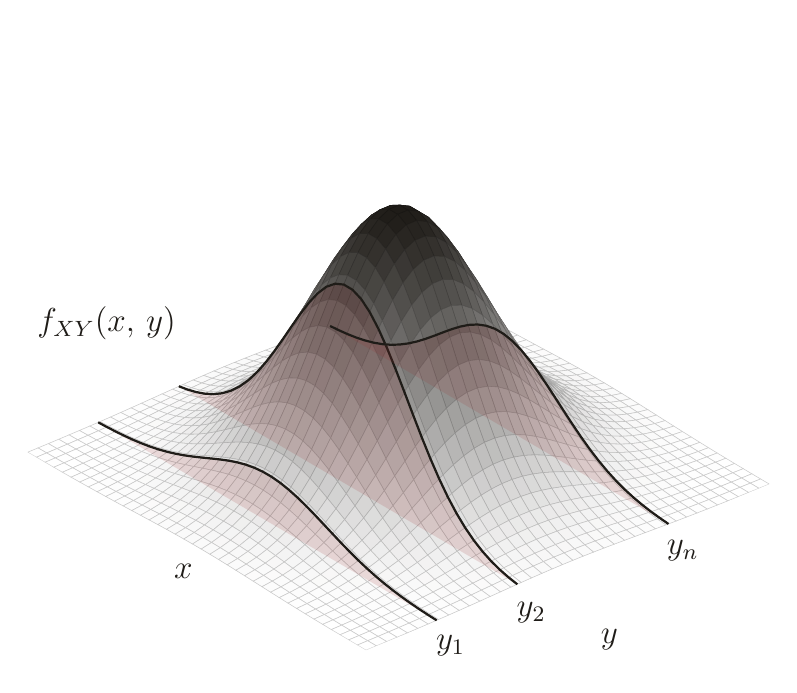
\begin{tikzpicture}[
    declare function={mu1=2;},
    declare function={mu2=2;},
    declare function={sigma1=1;},
    declare function={sigma2=1;},
    declare function={bivar(\ma,\sa,\mb,\sb)=
        1/(2*pi*\sa*\sb) * exp(-((x-\ma)^2/\sa^2 + (y-\mb)^2/\sb^2))/2;},
    declare function={slice(\yy)=
        1/(2*pi) * exp(-((x-2)^2 + (\yy-2)^2))/2;}]
\begin{axis}[
    axis line style={draw=none},
    colormap name=journalgray,
    width=11cm,
    view={50}{45},
    enlargelimits=false,
    domain=0:4,
    y domain=0:4,
    samples=40,
    xlabel=$x$,
    ylabel=$y$,
    zlabel={$f_{XY}(x,\,y)$},
    label style={journalink, font=\large},
    tick label style={journalink, font=\large},
    %% 座標軸線不畫，預設的框線刻度會在遠端浮成三個孤立的短記號，故一併關掉
    tick style={draw=none},
    xtick=\empty,
    ytick={0.7, 1.5, 3},
    yticklabels={$y_1$, $y_2$, $y_n$},
    ztick=\empty,
    zlabel style={rotate=-90, anchor=west},
]
\addplot3[surf, draw=journalink, line width=0.2pt] {bivar(mu1,sigma1,mu2,sigma2)};

%% 三片薄片: 每一片是聯合 pdf 在該 y 上沿 x 方向的截面，
%% 即 X 給定 Y=y 的條件分配 (尚未除以邊際密度)。
\addplot3[domain=0:4, samples y=0, samples=40, draw=journalmuted,
          line width=0.5pt, fill=journalaccent, fill opacity=0.15]
         (x, 0.7, {slice(0.7)});
\addplot3[domain=0:4, samples y=0, samples=40, journalink, line width=0.8pt]
         (x, 0.7, {slice(0.7)});

\addplot3[domain=0:4, samples y=0, samples=40, draw=journalmuted,
          line width=0.5pt, fill=journalaccent, fill opacity=0.15]
         (x, 1.5, {slice(1.5)});
\addplot3[domain=0:4, samples y=0, samples=40, journalink, line width=0.8pt]
         (x, 1.5, {slice(1.5)});

\addplot3[domain=0:4, samples y=0, samples=40, draw=journalmuted,
          line width=0.5pt, fill=journalaccent, fill opacity=0.15]
         (x, 3, {slice(3)});
\addplot3[domain=0:4, samples y=0, samples=40, journalink, line width=0.8pt]
         (x, 3, {slice(3)});
\end{axis}
\end{tikzpicture}
\end{document}
'
%   dvisvgm -O -d2 -n -o ../../images/teaching-topics/regression-function-surface.svg regression-function-surface.dvi

\documentclass[tikz,border=2pt]{standalone}
\usepackage{amsmath}
\usepackage{amssymb}
\usepackage{xcolor}
\usepackage{pgfplots}
\pgfplotsset{compat=1.18}

\definecolor{journalink}{HTML}{1F1C18}
\definecolor{journalmuted}{HTML}{8A7F72}
\definecolor{journalaccent}{HTML}{9C2D2D}

%% 12pt (即 \large) 之下的 script 級撐到 10pt，
%% 使 f 的下標與 y 的下標在 350px 顯示寬之下仍在 11px 之上。
\DeclareMathSizes{12}{12}{10}{8}

%% 書稿用 whitegray 灰階曲面; 本站改用同一色相的墨色濃淡，
%% 與其他圖的主線色 journalink 相稱。
\pgfplotsset{
  colormap={journalgray}{color(0cm)=(white); color(1cm)=(journalink)}
}

\begin{document}
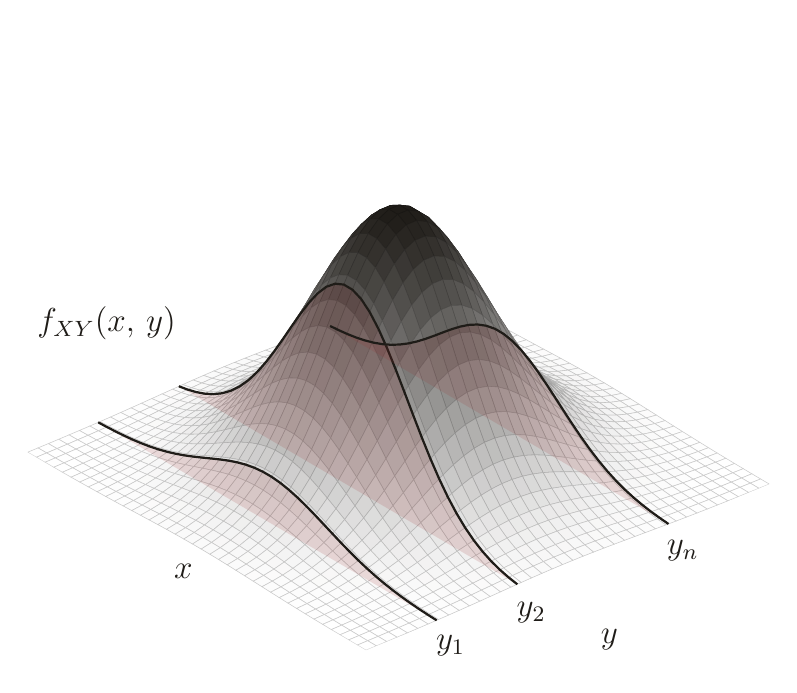
\begin{tikzpicture}[
    declare function={mu1=2;},
    declare function={mu2=2;},
    declare function={sigma1=1;},
    declare function={sigma2=1;},
    declare function={bivar(\ma,\sa,\mb,\sb)=
        1/(2*pi*\sa*\sb) * exp(-((x-\ma)^2/\sa^2 + (y-\mb)^2/\sb^2))/2;},
    declare function={slice(\yy)=
        1/(2*pi) * exp(-((x-2)^2 + (\yy-2)^2))/2;}]
\begin{axis}[
    axis line style={draw=none},
    colormap name=journalgray,
    width=11cm,
    view={50}{45},
    enlargelimits=false,
    domain=0:4,
    y domain=0:4,
    samples=40,
    xlabel=$x$,
    ylabel=$y$,
    zlabel={$f_{XY}(x,\,y)$},
    label style={journalink, font=\large},
    tick label style={journalink, font=\large},
    %% 座標軸線不畫，預設的框線刻度會在遠端浮成三個孤立的短記號，故一併關掉
    tick style={draw=none},
    xtick=\empty,
    ytick={0.7, 1.5, 3},
    yticklabels={$y_1$, $y_2$, $y_n$},
    ztick=\empty,
    zlabel style={rotate=-90, anchor=west},
]
\addplot3[surf, draw=journalink, line width=0.2pt] {bivar(mu1,sigma1,mu2,sigma2)};

%% 三片薄片: 每一片是聯合 pdf 在該 y 上沿 x 方向的截面，
%% 即 X 給定 Y=y 的條件分配 (尚未除以邊際密度)。
\addplot3[domain=0:4, samples y=0, samples=40, draw=journalmuted,
          line width=0.5pt, fill=journalaccent, fill opacity=0.15]
         (x, 0.7, {slice(0.7)});
\addplot3[domain=0:4, samples y=0, samples=40, journalink, line width=0.8pt]
         (x, 0.7, {slice(0.7)});

\addplot3[domain=0:4, samples y=0, samples=40, draw=journalmuted,
          line width=0.5pt, fill=journalaccent, fill opacity=0.15]
         (x, 1.5, {slice(1.5)});
\addplot3[domain=0:4, samples y=0, samples=40, journalink, line width=0.8pt]
         (x, 1.5, {slice(1.5)});

\addplot3[domain=0:4, samples y=0, samples=40, draw=journalmuted,
          line width=0.5pt, fill=journalaccent, fill opacity=0.15]
         (x, 3, {slice(3)});
\addplot3[domain=0:4, samples y=0, samples=40, journalink, line width=0.8pt]
         (x, 3, {slice(3)});
\end{axis}
\end{tikzpicture}
\end{document}
